% Weekly Status Report — Spectral Correlation with Event Cameras
% Compile: pdflatex weekly_report_2026-09-18.tex (twice, for the TOC-free cross-refs)
\documentclass[11pt,a4paper]{article}

\usepackage[T1]{fontenc}
\usepackage[utf8]{inputenc}
\usepackage{lmodern}
\usepackage[margin=2.2cm,top=2.4cm,bottom=2.6cm]{geometry}
\usepackage{amsmath,amssymb}
\usepackage{booktabs}
\usepackage{graphicx}
\usepackage{xcolor}
\usepackage[font=small,labelfont=bf,skip=4pt]{caption}
\usepackage{microtype}
\usepackage{enumitem}
\usepackage{tgheros}
\usepackage[hidelinks,colorlinks=true,linkcolor=reportblue,urlcolor=reportblue,citecolor=reportblue]{hyperref}

\definecolor{reportblue}{HTML}{1F3864}
\definecolor{accent}{HTML}{2E74B5}
\definecolor{pale}{HTML}{DDEBF7}
\definecolor{warn}{HTML}{B3470A}

\newcommand{\heading}[1]{\subsection*{\color{reportblue}#1}}
\newcommand{\subheading}[1]{\subsubsection*{\color{accent}#1}}
\newcommand{\qbox}[2]{%
  \par\medskip\noindent
  \fcolorbox{accent}{pale}{\parbox{\dimexpr\linewidth-2\fboxsep-2\fboxrule}{%
    \textbf{\textsf{\color{reportblue}#1}}\\[2pt]\itshape #2}}%
  \par\medskip}

\setlist[itemize]{itemsep=2pt,topsep=3pt}
\setlist[enumerate]{itemsep=3pt,topsep=3pt}

\title{\vspace{-1.2cm}\textsf{\color{reportblue}\Large Weekly Status Report}\\[2pt]
\textsf{\color{accent}\large Spectral Correlation with Event Cameras}}
\author{\textsf{Rich Baird \quad$\cdot$\quad for rmenon (PI)}}
\date{\textsf{Week of September 14--18, 2026}}

\begin{document}
\maketitle
\vspace{-1.4cm}

\begin{center}
\fcolorbox{reportblue}{white}{\parbox{0.96\textwidth}{%
\textsf{\textbf{\color{reportblue}TL;DR}\quad
The cross-color correlation is flat in effective frame rate ($10 \to 10{,}000$~FPS) and
grows only with total averaging time $T$ --- confirming ``it's not the FPS, it's the total
duration.'' The apparent FPS dependence in the earlier data was an artifact of how events
were binned, now fixed by switching to the paper's $\mathrm{ON}-\mathrm{OFF}$ estimator,
which also raises the converged correlation from $0.61$ to $0.78$. Single frames are
detectable but are not reliable \emph{estimators} of the spectral pattern; $\geq 5$ averaged
frames converge. The 60~Hz display caps scene dynamics, so the rotating-wheel experiment
is the right next step --- proposed protocol and predicted scaling inside.}}}
\end{center}

\tableofcontents
\vspace{0.4cm}

% ============================================================
\heading{1\quad Definitions --- aligning on terms first}

\begin{table}[h!]
\centering
\renewcommand{\arraystretch}{1.25}
\begin{tabular}{@{}clp{8.6cm}@{}}
\toprule
\textbf{Symbol} & \textsf{Name} & \textsf{Definition} \\
\midrule
$t$ & accumulation interval & wall-clock time integrated into one binned frame \\
$1/t$ & effective frame rate (FPS) & binned frames produced per second \\
$N$ & frame count & number of binned frames averaged \\
$T$ & total averaging time & $T = N \cdot t$ \\
$r$ & cross-color Pearson $r$ & correlation between the averaged frames of two wavelength recordings \\
$c$ & noise ceiling & within-recording reliability (split-half, Spearman--Brown) \\
\bottomrule
\end{tabular}
\end{table}

\medskip
One correction to the proposed definition ``effective frame rate $=$ number of frames $/$
accumulation time per frame'': with $N$ frames each accumulated over $t$, that expression
is $N/t$, which mixes units. The natural pair is
\[
\mathrm{FPS} = \frac{1}{t}, \qquad N = \frac{T}{t},
\]
so the two free knobs are $(T, \mathrm{FPS})$ and $N$ follows. This matters because the
central finding is that \textbf{$T$ is the operative variable and FPS is nearly free}.
Under these definitions the TL;DR example from the thread --- 1{,}000 frames at
10{,}000~FPS vs.\ 100 frames at 1{,}000~FPS, both $T = 100$~ms --- verifies exactly:
measured $r = -0.0043$ vs.\ $-0.0045$ (indistinguishable; both at the noise floor, since
$100$~ms is far below the $\sim$0.5~s minimum), and at $T = 5$~s, $r = 0.7847$ vs.\
$0.7844$.

% ============================================================
\heading{2\quad Responses to the open questions}

\qbox{Q1 --- ``Are you saying single events (very short durations) cannot be detected?
That is exactly what the DVS is used for (e.g.\ lightning) and Ca spikes (the BU paper).''}
{No --- and this is the distinction I failed to make in the thread. \textbf{Detection and
estimation are different problems.}}

Every threshold crossing is detected and timestamped at microsecond resolution; nothing in
our pipeline suppresses single events, which is exactly why DVS works for lightning and
Ca transients.

Our task, however, is \emph{estimation}: reconstructing the spatial diffraction pattern
that encodes the spectrum from binned events. A single event, or a single binned frame, is
one Poisson-distributed, threshold-quantized sample of that pattern. Quantitatively, in the
paper's event model a binned frame of window length $t$ estimates the log-intensity change
$\Delta \log I$ with error bounded by the contrast threshold $C$ (their Supplement~S4,
Lemma~S4.1):
\[
\sum_{i=1}^{n} p_i \;=\; \frac{1}{C}\bigl(f(t_{\mathrm{end}}) - f(t_{\mathrm{start}})\bigr) + \varepsilon,
\qquad |\varepsilon| < 1,
\]
and summing over $N$ windows of a total period $T$ with a scaling factor $a = C$:
\[
\Delta \log I \;=\; a \cdot \sum_{T} \sum_{t} e(x,y,t,p) \;-\; \sum_{i=1}^{N}\varepsilon_i,
\qquad |\varepsilon_i| < 1 .
\]
The residuals $\varepsilon_i$ of independent windows are roughly independent, so the
$N$-frame average carries error $\sim C/\sqrt{N}$ where a single frame carries a worst-case
$C$. This is the mechanism behind both our measured multi-frame floor and the paper's
Figure~2 (``large $N$ nearly recovers $L$''). Measured deviations of the reconstruction
from the converged answer: \textbf{1--2 frames deviate by up to ${\sim}0.74$} in correlation
units; \textbf{$\geq 5$ averaged frames converge ($\leq 0.075$)}. The BU paper makes the
same move from the tracking side: every frame is the sum of 16 refresh cycles, and their
ablation without accumulation degrades tracking RMSE by $+45\%$ (neural phase mask) and
$+54\%$ (neural amplitude mask).

\qbox{Q2 --- ``Maybe you mean the spectral reconstruction error increases with effective
frame rate (this is what I expect) and you have the data to show this.''}
{Measured this week --- the data shows \textbf{neither}. At fixed total averaging time,
reconstruction quality is essentially \textbf{flat in effective frame rate}. What increases
error is \textbf{less total averaging time}.}

\begin{table}[h!]
\centering
\caption{Mean cross-color Pearson $r$, $\mathrm{ON}-\mathrm{OFF}$ estimator, at fixed total
averaging time $T$ vs.\ effective frame rate (LCD circle recordings).}
\renewcommand{\arraystretch}{1.2}
\begin{tabular}{@{}lcccc@{}}
\toprule
$T$ & 10 FPS & 1{,}000 FPS & 10{,}000 FPS & FPS spread \\
\midrule
5~s   & 0.7796 & 0.7844 & 0.7847 & 0.005 \\
2~s   & 0.5675 & 0.5840 & 0.5847 & 0.017 \\
1~s   & 0.3410 & 0.3605 & 0.3614 & 0.020 \\
0.5~s & ---    & 0.1582 & 0.1588 & 0.001 \\
\bottomrule
\end{tabular}
\end{table}

There \emph{was} an apparent FPS dependence in the earlier data --- up to $11.6\%$ spread,
in the direction you found counter-intuitive --- but it was an artifact of folding
$\mathrm{ON}$ and $\mathrm{OFF}$ events into one count before a nonlinearity. Binning with
the paper's signed scheme ($\mathrm{ON}-\mathrm{OFF}$, which their Supplement proves
approximates $\Delta\log I$) collapses the spread to $0.5$--$2\%$, and it also
\emph{raises} the converged signal itself: $r(5\,\mathrm{s}) = 0.61 \to 0.78$, with
green--red reaching $0.90$. The $80\%$ cross-color separation target --- previously
reported as unreachable --- is now reached.

\qbox{Q3 --- ``This is spectroscopy, there is no FoV; cross-correlation across the colors
should be as low as possible. If it decreases with effective frame rate, does that mean
colors differentiate better as you go faster? Counter-intuitive.''}
{Two clarifications: on FoV, and on the counter-intuitive reading.}

\begin{enumerate}
\item \textbf{On ``no FoV'':} agreed the deliverable is the spectrum / RGB value. The
sensor's pixel array is still the substrate that encodes it --- the diffraction pattern is
spatial, and the binned frame is the intermediate representation from which the spectrum is
decoded. ``Across the full aperture'' in my earlier message meant: the estimator needs the
event record covering the whole encoding pattern, not a spatial subset. The output remains
a spectrum, not an image.
\item \textbf{On the counter-intuitive trend: your instinct was correct --- it was a trap.}
Cross-color $r$ falling toward zero is only \emph{better differentiation} if each recording
is independently reliable. Below ${\sim}0.25$~s of total averaging the recordings are not
yet self-reproducible; the low $r$ there is uncorrelated noise, not signal (as noted in the
thread: ``the lowest numbers are only just purely uncorrelated noise --- not signal''). The
correct statement is
\[
\text{differentiation} \;=\; \text{low cross-color } r \;\text{relative to a high noise ceiling } c,
\]
and the ceiling $c$ itself is built by total averaging time. Under the corrected estimator
the FPS curve is flat --- so no, FPS does not buy differentiation; total signal does.
\end{enumerate}

\qbox{Q4 --- ``Can you plot the cross-correlation as a function of the effective frame
rate?''}{Yes --- Figure~\ref{fig:fps}.}

\begin{figure}[h!]
\centering
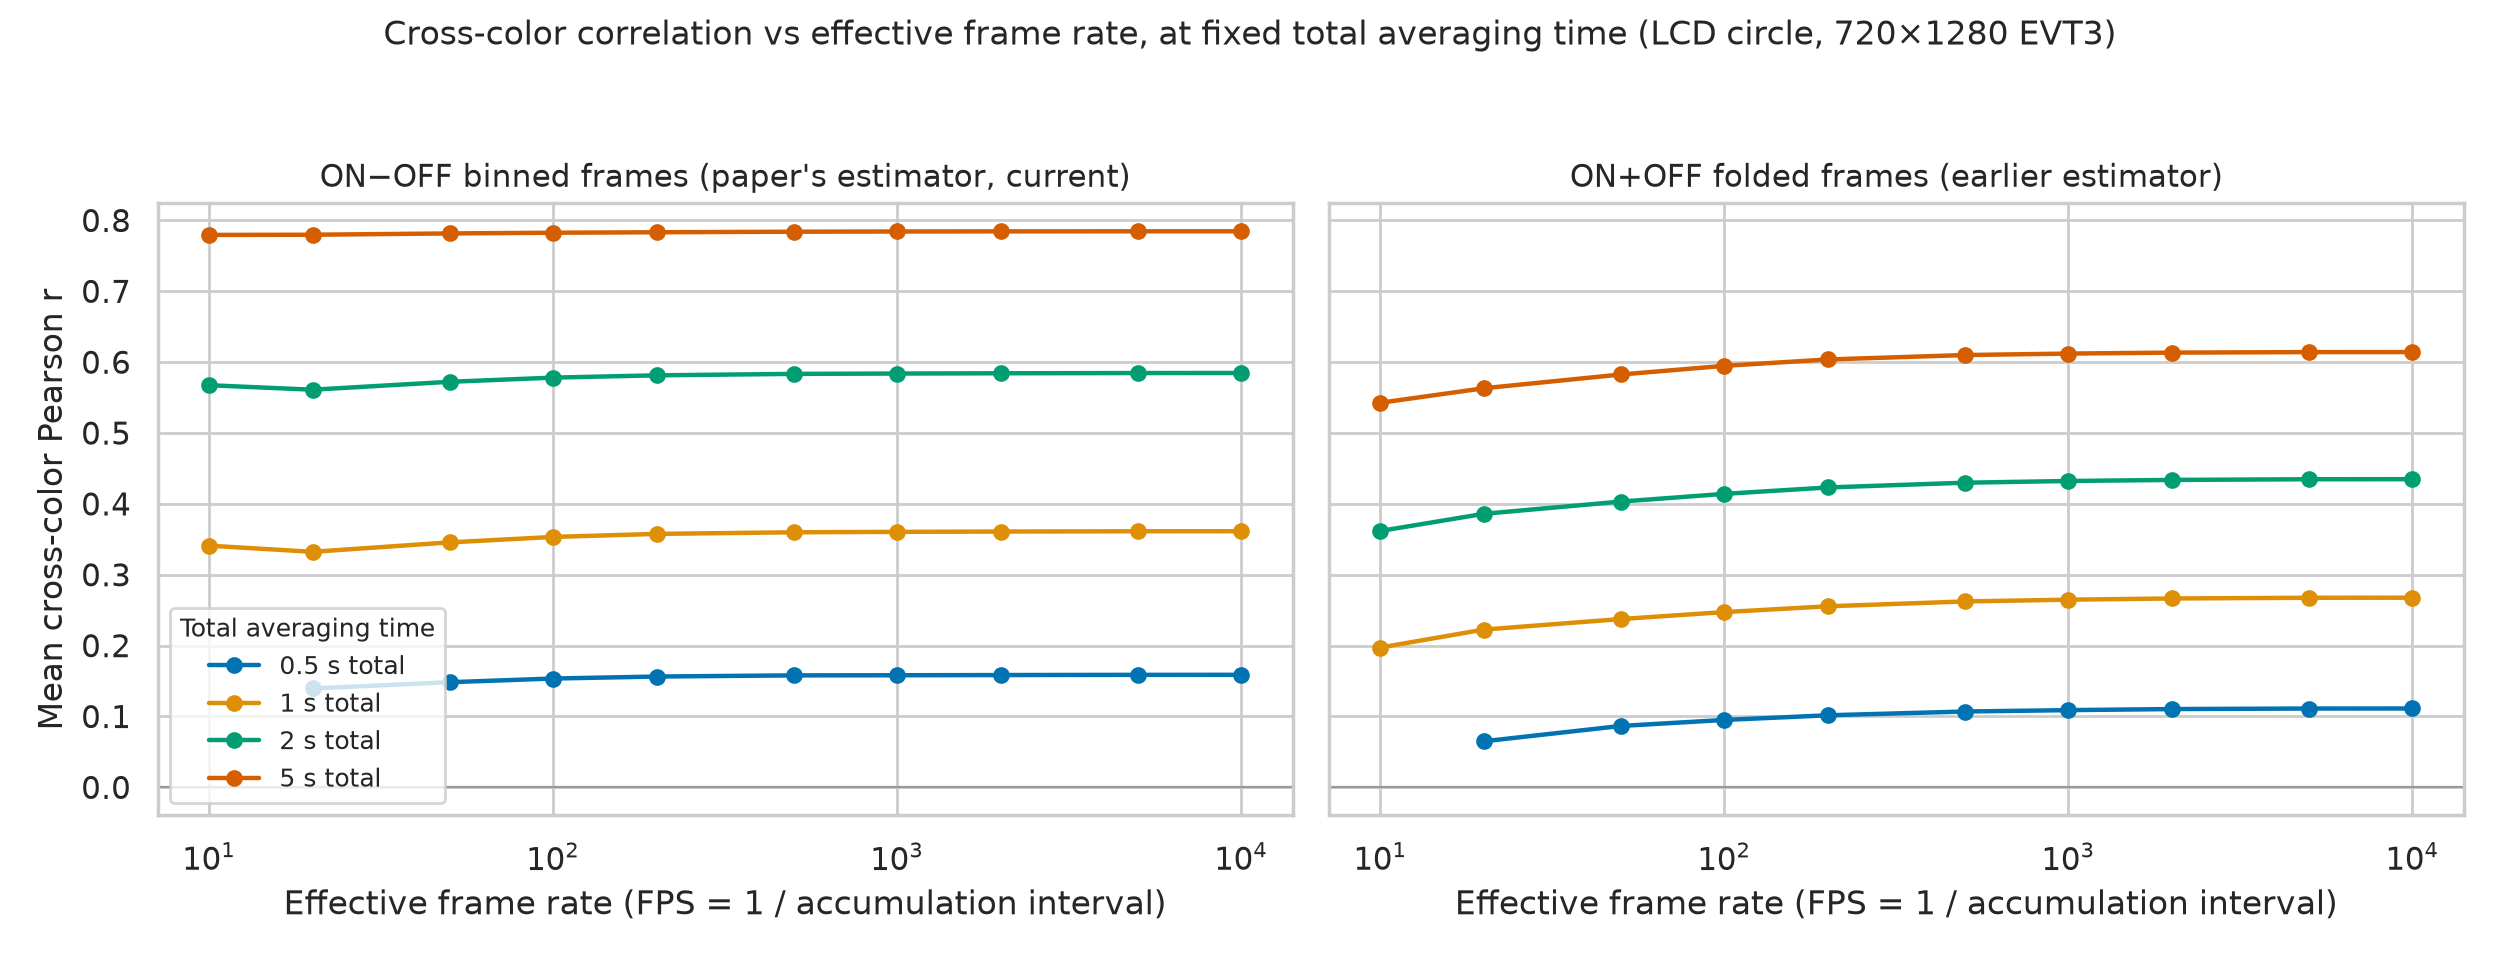
\includegraphics[width=\textwidth]{../reports/figures/cross_correlation_vs_effective_frame_rate.png}
\caption{\textsf{Mean cross-color Pearson $r$ vs.\ effective frame rate at fixed total
averaging times. \textbf{Left:} $\mathrm{ON}-\mathrm{OFF}$ binned frames (paper's
estimator, current). \textbf{Right:} earlier $\mathrm{ON}+\mathrm{OFF}$ folded estimator ---
this is where the apparent FPS trend lived, and the panel makes visible that it was an
artifact. Both panels share the $y$-axis; each curve is a fixed total averaging time
($0.5 / 1 / 2 / 5$~s); the $x$-axis spans effective FPS from 10 to 10{,}000.}}
\label{fig:fps}
\end{figure}

\qbox{Q5 --- ``Oh so you mean the display is not bright enough?''}
{No --- brightness is not the limiter. The display is a \textbf{60~Hz screen}: content
updates every $16.7$~ms, and the backlight/refresh modulates the sensor even for static
content.}

Measured consequences this week:
\begin{itemize}
\item The first accumulation interval containing reproducible structure is
\textbf{${\sim}16$~ms --- one display period} --- which we now treat as a display-period
artifact, not a fundamental limit. (The BU paper's ``16 frames at 1~ms'' coincidence is
worth re-examining on hardware that is not refresh-locked.)
\item Split-half reliability diagnostics go negative in a pattern consistent with windows
sampling fixed phases of a ${\sim}60$~Hz-periodic modulation.
\item Practical upshot: the \emph{scene's} temporal dynamics are capped by the display, so
the ``how fast can the scene change'' axis cannot be probed on this source --- hence the
rotating-wheel experiment below.
\end{itemize}

\qbox{Q6 --- ``With a faster source you can probe the limit I am looking for, right?
Rotating filter wheel with a lamp or bright source; add color filters for different
spectra?''}{Agreed --- that is the right next experiment, and it directly tests the claim
that smaller accumulation intervals require more dynamic signal. One design upgrade to
consider.}

Rather than a continuously rotating \emph{filter} wheel, the already-CAD'd 18-LED chopper
wheel (63~mm, $20^\circ$ station spacing, \texttt{models/}) puts the timing under precise
control: mounting two wavelength LEDs in the wheel gives a known, stable modulation
frequency \emph{and} the spectral pair in the same instrument, with the same correlation
pipeline as output.

The predicted scaling follows from the event-rate physics: a pixel fires when the
log-intensity change accumulates past the contrast threshold $C$, so a window of length $t$
captures roughly
\[
n_{\mathrm{events}} \;\approx\; \frac{t\,\lvert \mathrm{d}\log I / \mathrm{d}t \rvert}{C}
\]
events per active pixel. Enough events per window requires
\[
t_{\min} \;\approx\; \text{a few} \cdot \frac{C}{\lvert \mathrm{d}\log I/\mathrm{d}t \rvert}
\quad\Longrightarrow\quad t_{\min} \propto \frac{1}{f}\,,
\]
i.e.\ \textbf{the minimum usable accumulation interval scales inversely with the modulation
frequency}. Equivalently: the governing quantity is \textbf{events per window}, not FPS.

\emph{Protocol:}
\begin{enumerate}
\item Frequency ladder incommensurate with 60~Hz (e.g., 97, 211, 503~Hz) + one deliberate
60~Hz-commensurate run as a positive control for aliasing.
\item Chopper-off baseline capture: characterizes the display's intrinsic modulation and
provides the event-starved (``static scene'') end point, where $t_{\min}$ should blow up.
\item For each frequency: 10~s recording, full sweep with $\mathrm{ON}-\mathrm{OFF}$
binning; extract events-per-window, minimum $t$ with significant $r$, and the
FPS-invariance check.
\end{enumerate}
If the $t_{\min} \propto 1/f$ scaling holds --- equivalently, if results collapse onto a
single curve in events-per-window --- that confirms ``smaller $t$ requires faster dynamics''
quantitatively and gives the $t$-vs-frequency design map for the spectroscopy experiments.

\qbox{Q7 --- ``If you need more frames, we can define the effective frame rate accordingly:
number of frames / accumulation time per frame.''}
{Agreed on precise definitions --- proposal in \S1: $\mathrm{FPS} = 1/t$, $T = N \cdot t$,
$N = T \cdot \mathrm{FPS}$. Under these, the TL;DR example verifies exactly (numbers in
\S1).}

% ============================================================
\heading{3\quad Accomplishments this week}

\begin{itemize}
\item Completed the fine duration $\times$ frame-rate sweep instrument: 12--25~ms resolution
grid, $\mathrm{ON}-\mathrm{OFF}$ / ON / OFF / folded polarity modes, split-half noise
ceiling, per-pair Student-$t$ significance.
\item Switched the estimator to the BU paper's $\mathrm{ON}-\mathrm{OFF}$ binning (proven
$\approx \Delta\log I$, their Supplement~S4): converged cross-color correlation
$0.61 \to 0.78$, green--red $0.90$; the $80\%$ separation target is now reached.
\item Diagnosed the earlier FPS-dependent trend as a polarity-folding artifact; FPS spread
collapsed from $11.6\%$ to $0.5$--$2\%$.
\item Verified all four shared claims against Shah et al.\ (CVPR 2024), including their
16-refresh-cycle binning and their no-accumulation ablation ($+45$--$54\%$ RMSE) matching
our multi-frame requirement.
\item Produced Figure~1 (the requested cross-correlation vs.\ effective-frame-rate plot);
verification report deck delivered (\texttt{results/polarity\_verification\_report.pptx}).
\end{itemize}

\heading{4\quad In progress}

\begin{table}[h!]
\centering
\renewcommand{\arraystretch}{1.2}
\begin{tabular}{@{}p{7.6cm}p{4.2cm}p{4.2cm}@{}}
\toprule
\textsf{Task} & \textsf{Status} & \textsf{Expected completion} \\
\midrule
Chopper LED wheel mounting + frequency ladder captures & hardware ready, awaiting bench time & next week \\
Partition-invariance test ($\mathrm{ON}-\mathrm{OFF}$, linear scaling; no new capture needed) & queued & early next week \\
Sub-10-frame floor re-measurement under the corrected estimator & queued & next week \\
\bottomrule
\end{tabular}
\end{table}

\heading{5\quad Blockers}

\textbf{60~Hz display ceiling} --- the current source cannot probe scene dynamics above one
refresh period, and it injects its own periodic modulation (the likely cause of a negative
reliability diagnostic in the split-half analysis). Impact: the $t_{\min}$-vs-frequency
scaling cannot be measured on the LCD. Resolution: the chopper/LED wheel captures above ---
hardware exists, needs mounting.

\heading{6\quad Next week's priorities}

\begin{enumerate}
\item Chopper bench setup; frequency ladder captures (incommensurate with 60~Hz + one
commensurate control + chopper-off baseline).
\item Partition-invariance test on existing recordings (validates the estimator before new
captures are analyzed).
\item $t_{\min} \propto 1/f$ scaling analysis from the frequency ladder; updated FPS plot
with chopper data.
\item Revised spectra-deck conclusions ($80\%$ target reached; 16~ms finding re-scoped as a
display-period artifact pending chopper data).
\end{enumerate}

\heading{7\quad Standing operating envelope (from this week's measurements)}

\begin{center}
\renewcommand{\arraystretch}{1.2}
\fcolorbox{accent}{pale}{\parbox{0.94\textwidth}{\centering
$\geq 5$ averaged frames; \quad $\geq 0.5$--$1$~s total averaging for reliable
discrimination; \quad effective FPS free from 10 to 10{,}000.\\[2pt]
\small The paper's 16~ms bin sits at the lower \emph{edge} of detectability on
display-driven content; treat it as an edge, not an operating point, until the chopper
data re-baselines it.}}
\end{center}

\medskip
\textsf{\small Data: LCD circle recordings, $720\times1280$ EVT3, 5~s per color; crop +
spatial high-pass + support-masked Pearson; $\mathrm{ON}-\mathrm{OFF}$ binning per Shah et
al.\ Supplement~S4. Scripts and result tables in
\texttt{src/hypercam/}\allowbreak\texttt{duration\_sweep.py} and
\texttt{src/hypercam/}\allowbreak\texttt{results/}.}

\end{document}
